\documentclass[1p]{elsarticle_modified}
%\bibliographystyle{elsarticle-num}

%\usepackage[colorlinks]{hyperref}
%\usepackage{abbrmath_seonhwa} %\Abb, \Ascr, \Acal ,\Abf, \Afrak
\usepackage{amsfonts}
\usepackage{amssymb}
\usepackage{amsmath}
\usepackage{amsthm}
\usepackage{scalefnt}
\usepackage{amsbsy}
\usepackage{kotex}
\usepackage{caption}
\usepackage{subfig}
\usepackage{color}
\usepackage{graphicx}
\usepackage{xcolor} %% white, black, red, green, blue, cyan, magenta, yellow
\usepackage{float}
\usepackage{setspace}
\usepackage{hyperref}

\usepackage{tikz}
\usetikzlibrary{arrows}

\usepackage{multirow}
\usepackage{array} % fixed length table
\usepackage{hhline}

%%%%%%%%%%%%%%%%%%%%%
\makeatletter
\renewcommand*\env@matrix[1][\arraystretch]{%
	\edef\arraystretch{#1}%
	\hskip -\arraycolsep
	\let\@ifnextchar\new@ifnextchar
	\array{*\c@MaxMatrixCols c}}
\makeatother %https://tex.stackexchange.com/questions/14071/how-can-i-increase-the-line-spacing-in-a-matrix
%%%%%%%%%%%%%%%

\usepackage[normalem]{ulem}

\newcommand{\msout}[1]{\ifmmode\text{\sout{\ensuremath{#1}}}\else\sout{#1}\fi}
%SOURCE: \msout is \stkout macro in https://tex.stackexchange.com/questions/20609/strikeout-in-math-mode

\newcommand{\cancel}[1]{
	\ifmmode
	{\color{red}\msout{#1}}
	\else
	{\color{red}\sout{#1}}
	\fi
}

\newcommand{\add}[1]{
	{\color{blue}\uwave{#1}}
}

\newcommand{\replace}[2]{
	\ifmmode
	{\color{red}\msout{#1}}{\color{blue}\uwave{#2}}
	\else
	{\color{red}\sout{#1}}{\color{blue}\uwave{#2}}
	\fi
}

\newcommand{\Sol}{\mathcal{S}} %segment
\newcommand{\D}{D} %diagram
\newcommand{\A}{\mathcal{A}} %arc


%%%%%%%%%%%%%%%%%%%%%%%%%%%%%5 test

\def\sl{\operatorname{\textup{SL}}(2,\Cbb)}
\def\psl{\operatorname{\textup{PSL}}(2,\Cbb)}
\def\quan{\mkern 1mu \triangleright \mkern 1mu}

\theoremstyle{definition}
\newtheorem{thm}{Theorem}[section]
\newtheorem{prop}[thm]{Proposition}
\newtheorem{lem}[thm]{Lemma}
\newtheorem{ques}[thm]{Question}
\newtheorem{cor}[thm]{Corollary}
\newtheorem{defn}[thm]{Definition}
\newtheorem{exam}[thm]{Example}
\newtheorem{rmk}[thm]{Remark}
\newtheorem{alg}[thm]{Algorithm}

\newcommand{\I}{\sqrt{-1}}
\begin{document}

%\begin{frontmatter}
%
%\title{Boundary parabolic representations of knots up to 8 crossings}
%
%%% Group authors per affiliation:
%\author{Yunhi Cho} 
%\address{Department of Mathematics, University of Seoul, Seoul, Korea}
%\ead{yhcho@uos.ac.kr}
%
%
%\author{Seonhwa Kim} %\fnref{s_kim}}
%\address{Center for Geometry and Physics, Institute for Basic Science, Pohang, 37673, Korea}
%\ead{ryeona17@ibs.re.kr}
%
%\author{Hyuk Kim}
%\address{Department of Mathematical Sciences, Seoul National University, Seoul 08826, Korea}
%\ead{hyukkim@snu.ac.kr}
%
%\author{Seokbeom Yoon}
%\address{Department of Mathematical Sciences, Seoul National University, Seoul, 08826,  Korea}
%\ead{sbyoon15@snu.ac.kr}
%
%\begin{abstract}
%We find all boundary parabolic representation of knots up to 8 crossings.
%
%\end{abstract}
%\begin{keyword}
%    \MSC[2010] 57M25 
%\end{keyword}
%
%\end{frontmatter}

%\linenumbers
%\tableofcontents
%
\newcommand\colored[1]{\textcolor{white}{\rule[-0.35ex]{0.8em}{1.4ex}}\kern-0.8em\color{red} #1}%
%\newcommand\colored[1]{\textcolor{white}{ #1}\kern-2.17ex	\textcolor{white}{ #1}\kern-1.81ex	\textcolor{white}{ #1}\kern-2.15ex\color{red}#1	}

{\Large $\underline{11n_{55}~(K11n_{55})}$}

\setlength{\tabcolsep}{10pt}
\renewcommand{\arraystretch}{1.6}
\vspace{1cm}\begin{tabular}{m{100pt}>{\centering\arraybackslash}m{274pt}}
\multirow{5}{120pt}{
	\centering
	\includegraphics[width=112pt]{../../../GIT/diagram.site/Diagrams/png/671_11n_55.png}\\
\ \ \ A knot diagram\footnotemark}&
\allowdisplaybreaks
\textbf{Linearized knot diagam} \\
\cline{2-2}
 &
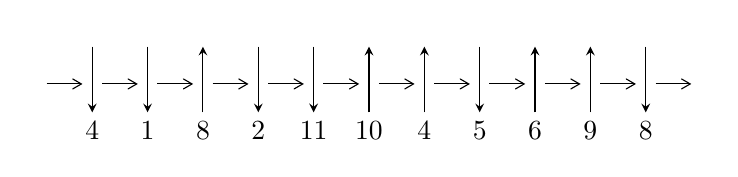
\begin{tikzpicture}[x=20pt, y=17pt]
	% nodes
	\node (C0) at (0, 0) {};
	\node (C1) at (1, 0) {};
	\node (C1U) at (1, +1) {};
	\node (C1D) at (1, -1) {4};

	\node (C2) at (2, 0) {};
	\node (C2U) at (2, +1) {};
	\node (C2D) at (2, -1) {1};

	\node (C3) at (3, 0) {};
	\node (C3U) at (3, +1) {};
	\node (C3D) at (3, -1) {8};

	\node (C4) at (4, 0) {};
	\node (C4U) at (4, +1) {};
	\node (C4D) at (4, -1) {2};

	\node (C5) at (5, 0) {};
	\node (C5U) at (5, +1) {};
	\node (C5D) at (5, -1) {11};

	\node (C6) at (6, 0) {};
	\node (C6U) at (6, +1) {};
	\node (C6D) at (6, -1) {10};

	\node (C7) at (7, 0) {};
	\node (C7U) at (7, +1) {};
	\node (C7D) at (7, -1) {4};

	\node (C8) at (8, 0) {};
	\node (C8U) at (8, +1) {};
	\node (C8D) at (8, -1) {5};

	\node (C9) at (9, 0) {};
	\node (C9U) at (9, +1) {};
	\node (C9D) at (9, -1) {6};

	\node (C10) at (10, 0) {};
	\node (C10U) at (10, +1) {};
	\node (C10D) at (10, -1) {9};

	\node (C11) at (11, 0) {};
	\node (C11U) at (11, +1) {};
	\node (C11D) at (11, -1) {8};
	\node (C12) at (12, 0) {};

	% arrows
	\draw[->,>={angle 60}]
	(C0) edge (C1) (C1) edge (C2) (C2) edge (C3) (C3) edge (C4) (C4) edge (C5) (C5) edge (C6) (C6) edge (C7) (C7) edge (C8) (C8) edge (C9) (C9) edge (C10) (C10) edge (C11) (C11) edge (C12) ;	\draw[->,>=stealth]
	(C1U) edge (C1D) (C2U) edge (C2D) (C3D) edge (C3U) (C4U) edge (C4D) (C5U) edge (C5D) (C6D) edge (C6U) (C7D) edge (C7U) (C8U) edge (C8D) (C9D) edge (C9U) (C10D) edge (C10U) (C11U) edge (C11D) ;
	\end{tikzpicture} \\
\hhline{~~} \\& 
\textbf{Solving Sequence} \\ \cline{2-2} 
 &
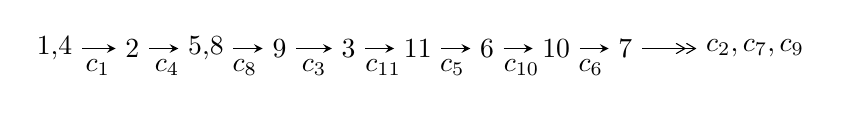
\begin{tikzpicture}[x=25pt, y=7pt]
	% node
	\node (A0) at (-1/8, 0) {1,4};
	\node (A1) at (1, 0) {2};
	\node (A2) at (33/16, 0) {5,8};
	\node (A3) at (25/8, 0) {9};
	\node (A4) at (33/8, 0) {3};
	\node (A5) at (41/8, 0) {11};
	\node (A6) at (49/8, 0) {6};
	\node (A7) at (57/8, 0) {10};
	\node (A8) at (65/8, 0) {7};
	\node (C1) at (1/2, -1) {$c_{1}$};
	\node (C2) at (3/2, -1) {$c_{4}$};
	\node (C3) at (21/8, -1) {$c_{8}$};
	\node (C4) at (29/8, -1) {$c_{3}$};
	\node (C5) at (37/8, -1) {$c_{11}$};
	\node (C6) at (45/8, -1) {$c_{5}$};
	\node (C7) at (53/8, -1) {$c_{10}$};
	\node (C8) at (61/8, -1) {$c_{6}$};
	\node (A9) at (10, 0) {$c_{2},c_{7},c_{9}$};

	% edge
	\draw[->,>=stealth]	
	(A0) edge (A1) (A1) edge (A2) (A2) edge (A3) (A3) edge (A4) (A4) edge (A5) (A5) edge (A6) (A6) edge (A7) (A7) edge (A8) ;
	\draw[->>,>={angle 60}]	
	(A8) edge (A9);
\end{tikzpicture} \\ 

\end{tabular} \\

\footnotetext{
The image of knot diagram is generated by the software ``\textbf{Draw programme}" developed by Andrew Bartholomew(\url{http://www.layer8.co.uk/maths/draw/index.htm\#Running-draw}), where we modified some parts for our purpose(\url{https://github.com/CATsTAILs/LinksPainter}).
}\phantom \\ \newline 
\centering \textbf{Ideals for irreducible components\footnotemark of $X_{\text{par}}$} 
 
\begin{align*}
I^u_{1}&=\langle 
-43 u^{35}-186 u^{34}+\cdots+32 b+285,\;41 u^{35}+278 u^{34}+\cdots+4 a+100,\;u^{36}+7 u^{35}+\cdots+7 u+1\rangle \\
I^u_{2}&=\langle 
b^6- b^5- b^4+2 b^3- b+1,\;a,\;u-1\rangle \\
\\
\end{align*}
\raggedright * 2 irreducible components of $\dim_{\mathbb{C}}=0$, with total 42 representations.\\
\footnotetext{All coefficients of polynomials are rational numbers. But the coefficients are sometimes approximated in decimal forms when there is not enough margin.}
\newpage
\renewcommand{\arraystretch}{1}
\centering \section*{I. $I^u_{1}= \langle -43 u^{35}-186 u^{34}+\cdots+32 b+285,\;41 u^{35}+278 u^{34}+\cdots+4 a+100,\;u^{36}+7 u^{35}+\cdots+7 u+1 \rangle$}
\flushleft \textbf{(i) Arc colorings}\\
\begin{tabular}{m{7pt} m{180pt} m{7pt} m{180pt} }
\flushright $a_{1}=$&$\begin{pmatrix}1\\0\end{pmatrix}$ \\
\flushright $a_{4}=$&$\begin{pmatrix}0\\u\end{pmatrix}$ \\
\flushright $a_{2}=$&$\begin{pmatrix}1\\u^2\end{pmatrix}$ \\
\flushright $a_{5}=$&$\begin{pmatrix}- u\\- u^3+u\end{pmatrix}$ \\
\flushright $a_{8}=$&$\begin{pmatrix}-\frac{41}{4} u^{35}-\frac{139}{2} u^{34}+\cdots-126 u-25\\1.34375 u^{35}+5.81250 u^{34}+\cdots-28.4375 u-8.90625\end{pmatrix}$ \\
\flushright $a_{9}=$&$\begin{pmatrix}-12.5938 u^{35}-82.0625 u^{34}+\cdots-128.313 u-23.8438\\-0.906250 u^{35}-9.43750 u^{34}+\cdots-50.6875 u-13.9063\end{pmatrix}$ \\
\flushright $a_{3}=$&$\begin{pmatrix}- u^2+1\\u^2\end{pmatrix}$ \\
\flushright $a_{11}=$&$\begin{pmatrix}u\\0.0312500 u^{35}+0.187500 u^{34}+\cdots+1.18750 u+0.0312500\end{pmatrix}$ \\
\flushright $a_{6}=$&$\begin{pmatrix}-0.0312500 u^{35}-0.187500 u^{34}+\cdots-1.18750 u-0.0312500\\-0.906250 u^{35}-5.50000 u^{34}+\cdots-4.75000 u-0.968750\end{pmatrix}$ \\
\flushright $a_{10}=$&$\begin{pmatrix}-0.625000 u^{35}-3.81250 u^{34}+\cdots-4.06250 u+0.312500\\0.968750 u^{35}+5.87500 u^{34}+\cdots+6.12500 u+1.03125\end{pmatrix}$ \\
\flushright $a_{7}=$&$\begin{pmatrix}\frac{41}{4} u^{35}+\frac{139}{2} u^{34}+\cdots+126 u+25\\-2.84375 u^{35}-13.8125 u^{34}+\cdots+33.9375 u+11.1563\end{pmatrix}$\\ \flushright $a_{7}=$&$\begin{pmatrix}\frac{41}{4} u^{35}+\frac{139}{2} u^{34}+\cdots+126 u+25\\-2.84375 u^{35}-13.8125 u^{34}+\cdots+33.9375 u+11.1563\end{pmatrix}$\\&\end{tabular}
\flushleft \textbf{(ii) Obstruction class $= -1$}\\~\\
\flushleft \textbf{(iii) Cusp Shapes $= \frac{161}{16} u^{35}+\frac{897}{16} u^{34}+\cdots-\frac{87}{16} u-\frac{49}{8}$}\\~\\
\newpage\renewcommand{\arraystretch}{1}
\flushleft \textbf{(iv) u-Polynomials at the component}\newline \\
\begin{tabular}{m{50pt}|m{274pt}}
Crossings & \hspace{64pt}u-Polynomials at each crossing \\
\hline $$\begin{aligned}c_{1},c_{4}\end{aligned}$$&$\begin{aligned}
&u^{36}-7 u^{35}+\cdots-7 u+1
\end{aligned}$\\
\hline $$\begin{aligned}c_{2}\end{aligned}$$&$\begin{aligned}
&u^{36}+9 u^{35}+\cdots+11 u+1
\end{aligned}$\\
\hline $$\begin{aligned}c_{3},c_{7}\end{aligned}$$&$\begin{aligned}
&u^{36}- u^{35}+\cdots-128 u+64
\end{aligned}$\\
\hline $$\begin{aligned}c_{5}\end{aligned}$$&$\begin{aligned}
&u^{36}-6 u^{35}+\cdots-74 u+17
\end{aligned}$\\
\hline $$\begin{aligned}c_{6},c_{9}\end{aligned}$$&$\begin{aligned}
&u^{36}-2 u^{35}+\cdots-2 u+1
\end{aligned}$\\
\hline $$\begin{aligned}c_{8}\end{aligned}$$&$\begin{aligned}
&u^{36}+2 u^{35}+\cdots-56 u+49
\end{aligned}$\\
\hline $$\begin{aligned}c_{10}\end{aligned}$$&$\begin{aligned}
&u^{36}-18 u^{35}+\cdots-2 u+1
\end{aligned}$\\
\hline $$\begin{aligned}c_{11}\end{aligned}$$&$\begin{aligned}
&u^{36}-2 u^{35}+\cdots-2 u+1
\end{aligned}$\\
\hline
\end{tabular}\\~\\
\newpage\renewcommand{\arraystretch}{1}
\flushleft \textbf{(v) Riley Polynomials at the component}\newline \\
\begin{tabular}{m{50pt}|m{274pt}}
Crossings & \hspace{64pt}Riley Polynomials at each crossing \\
\hline $$\begin{aligned}c_{1},c_{4}\end{aligned}$$&$\begin{aligned}
&y^{36}-9 y^{35}+\cdots-11 y+1
\end{aligned}$\\
\hline $$\begin{aligned}c_{2}\end{aligned}$$&$\begin{aligned}
&y^{36}+43 y^{35}+\cdots+57 y+1
\end{aligned}$\\
\hline $$\begin{aligned}c_{3},c_{7}\end{aligned}$$&$\begin{aligned}
&y^{36}-39 y^{35}+\cdots-61440 y+4096
\end{aligned}$\\
\hline $$\begin{aligned}c_{5}\end{aligned}$$&$\begin{aligned}
&y^{36}+14 y^{35}+\cdots+2990 y+289
\end{aligned}$\\
\hline $$\begin{aligned}c_{6},c_{9}\end{aligned}$$&$\begin{aligned}
&y^{36}-18 y^{35}+\cdots-2 y+1
\end{aligned}$\\
\hline $$\begin{aligned}c_{8}\end{aligned}$$&$\begin{aligned}
&y^{36}+6 y^{35}+\cdots+490 y+2401
\end{aligned}$\\
\hline $$\begin{aligned}c_{10}\end{aligned}$$&$\begin{aligned}
&y^{36}+2 y^{35}+\cdots+18 y+1
\end{aligned}$\\
\hline $$\begin{aligned}c_{11}\end{aligned}$$&$\begin{aligned}
&y^{36}+42 y^{35}+\cdots-2 y+1
\end{aligned}$\\
\hline
\end{tabular}\\~\\
\newpage\flushleft \textbf{(vi) Complex Volumes and Cusp Shapes}
$$\begin{array}{c|c|c}  
\text{Solutions to }I^u_{1}& \I (\text{vol} + \sqrt{-1}CS) & \text{Cusp shape}\\
 \hline 
\begin{aligned}
u &= \phantom{-}1.061290 + 0.326287 I \\
a &= -0.642038 - 0.460220 I \\
b &= \phantom{-}0.303700 + 0.290509 I\end{aligned}
 & -0.00265 + 2.23213 I & -0.68244 - 4.15610 I \\ \hline\begin{aligned}
u &= \phantom{-}1.061290 - 0.326287 I \\
a &= -0.642038 + 0.460220 I \\
b &= \phantom{-}0.303700 - 0.290509 I\end{aligned}
 & -0.00265 - 2.23213 I & -0.68244 + 4.15610 I \\ \hline\begin{aligned}
u &= \phantom{-}0.515673 + 0.710660 I \\
a &= -0.862097 - 0.946791 I \\
b &= \phantom{-}0.155712 + 0.653329 I\end{aligned}
 & \phantom{-}2.02771 - 6.40530 I & \phantom{-}1.88436 + 7.11312 I \\ \hline\begin{aligned}
u &= \phantom{-}0.515673 - 0.710660 I \\
a &= -0.862097 + 0.946791 I \\
b &= \phantom{-}0.155712 - 0.653329 I\end{aligned}
 & \phantom{-}2.02771 + 6.40530 I & \phantom{-}1.88436 - 7.11312 I \\ \hline\begin{aligned}
u &= \phantom{-}0.785644 + 0.339119 I \\
a &= \phantom{-}0.531433 + 0.754793 I \\
b &= -0.166697 - 0.401361 I\end{aligned}
 & -1.48377 - 1.33270 I & -5.42230 + 4.02694 I \\ \hline\begin{aligned}
u &= \phantom{-}0.785644 - 0.339119 I \\
a &= \phantom{-}0.531433 - 0.754793 I \\
b &= -0.166697 + 0.401361 I\end{aligned}
 & -1.48377 + 1.33270 I & -5.42230 - 4.02694 I \\ \hline\begin{aligned}
u &= \phantom{-}1.177000 + 0.085808 I \\
a &= \phantom{-}0.589499 + 0.125039 I \\
b &= -0.316874 - 0.078348 I\end{aligned}
 & -2.50865 - 0.37469 I & -1.90153 - 1.63609 I \\ \hline\begin{aligned}
u &= \phantom{-}1.177000 - 0.085808 I \\
a &= \phantom{-}0.589499 - 0.125039 I \\
b &= -0.316874 + 0.078348 I\end{aligned}
 & -2.50865 + 0.37469 I & -1.90153 + 1.63609 I \\ \hline\begin{aligned}
u &= -0.888941 + 0.845189 I \\
a &= \phantom{-}0.755005 + 0.931742 I \\
b &= \phantom{-}0.44408 - 1.66748 I\end{aligned}
 & \phantom{-}3.30506 + 0.68404 I & -1.00000 + 0.503330 I \\ \hline\begin{aligned}
u &= -0.888941 - 0.845189 I \\
a &= \phantom{-}0.755005 - 0.931742 I \\
b &= \phantom{-}0.44408 + 1.66748 I\end{aligned}
 & \phantom{-}3.30506 - 0.68404 I & -1.00000 - 0.503330 I\\
 \hline 
 \end{array}$$\newpage$$\begin{array}{c|c|c}  
\text{Solutions to }I^u_{1}& \I (\text{vol} + \sqrt{-1}CS) & \text{Cusp shape}\\
 \hline 
\begin{aligned}
u &= \phantom{-}0.512682 + 0.569033 I \\
a &= \phantom{-}0.780897 + 0.985416 I \\
b &= -0.113983 - 0.584856 I\end{aligned}
 & -0.43379 - 1.94575 I & -1.80433 + 3.98828 I \\ \hline\begin{aligned}
u &= \phantom{-}0.512682 - 0.569033 I \\
a &= \phantom{-}0.780897 - 0.985416 I \\
b &= -0.113983 + 0.584856 I\end{aligned}
 & -0.43379 + 1.94575 I & -1.80433 - 3.98828 I \\ \hline\begin{aligned}
u &= \phantom{-}1.231010 + 0.192137 I \\
a &= -0.699294 - 0.225880 I \\
b &= \phantom{-}0.379504 + 0.152175 I\end{aligned}
 & -0.47071 - 4.51088 I & \phantom{-}0.51157 + 3.50709 I \\ \hline\begin{aligned}
u &= \phantom{-}1.231010 - 0.192137 I \\
a &= -0.699294 + 0.225880 I \\
b &= \phantom{-}0.379504 - 0.152175 I\end{aligned}
 & -0.47071 + 4.51088 I & \phantom{-}0.51157 - 3.50709 I \\ \hline\begin{aligned}
u &= -0.977681 + 0.835405 I \\
a &= -0.710165 - 0.943837 I \\
b &= -0.44152 + 1.76315 I\end{aligned}
 & \phantom{-}3.02757 + 5.62134 I & -1.94819 - 5.64508 I \\ \hline\begin{aligned}
u &= -0.977681 - 0.835405 I \\
a &= -0.710165 + 0.943837 I \\
b &= -0.44152 - 1.76315 I\end{aligned}
 & \phantom{-}3.02757 - 5.62134 I & -1.94819 + 5.64508 I \\ \hline\begin{aligned}
u &= \phantom{-}0.268102 + 0.646439 I \\
a &= -0.923789 - 1.064280 I \\
b &= \phantom{-}0.005979 + 0.692881 I\end{aligned}
 & \phantom{-}3.06250 + 1.09495 I & \phantom{-}4.73244 - 0.17091 I \\ \hline\begin{aligned}
u &= \phantom{-}0.268102 - 0.646439 I \\
a &= -0.923789 + 1.064280 I \\
b &= \phantom{-}0.005979 - 0.692881 I\end{aligned}
 & \phantom{-}3.06250 - 1.09495 I & \phantom{-}4.73244 + 0.17091 I \\ \hline\begin{aligned}
u &= -0.813768 + 1.033210 I \\
a &= \phantom{-}0.813317 + 1.002390 I \\
b &= \phantom{-}0.26375 - 1.59543 I\end{aligned}
 & \phantom{-}6.28852 - 0.72428 I & \phantom{-0.000000 } 0 \\ \hline\begin{aligned}
u &= -0.813768 - 1.033210 I \\
a &= \phantom{-}0.813317 - 1.002390 I \\
b &= \phantom{-}0.26375 + 1.59543 I\end{aligned}
 & \phantom{-}6.28852 + 0.72428 I & \phantom{-0.000000 } 0\\
 \hline 
 \end{array}$$\newpage$$\begin{array}{c|c|c}  
\text{Solutions to }I^u_{1}& \I (\text{vol} + \sqrt{-1}CS) & \text{Cusp shape}\\
 \hline 
\begin{aligned}
u &= -0.791993 + 1.084540 I \\
a &= -0.827522 - 1.018650 I \\
b &= -0.21954 + 1.58084 I\end{aligned}
 & \phantom{-}9.06514 - 5.65458 I & \phantom{-}3.21416 + 3.51542 I \\ \hline\begin{aligned}
u &= -0.791993 - 1.084540 I \\
a &= -0.827522 + 1.018650 I \\
b &= -0.21954 - 1.58084 I\end{aligned}
 & \phantom{-}9.06514 + 5.65458 I & \phantom{-}3.21416 - 3.51542 I \\ \hline\begin{aligned}
u &= -0.890160 + 1.056150 I \\
a &= -0.787704 - 1.021790 I \\
b &= -0.24615 + 1.66009 I\end{aligned}
 & \phantom{-}10.62450 + 2.78646 I & \phantom{-}4.96714 + 0. I\phantom{ +0.000000I} \\ \hline\begin{aligned}
u &= -0.890160 - 1.056150 I \\
a &= -0.787704 + 1.021790 I \\
b &= -0.24615 - 1.66009 I\end{aligned}
 & \phantom{-}10.62450 - 2.78646 I & \phantom{-}4.96714 + 0. I\phantom{ +0.000000I} \\ \hline\begin{aligned}
u &= -0.584281 + 0.166417 I \\
a &= \phantom{-}1.042350 + 0.296118 I \\
b &= \phantom{-}1.36445 - 0.54728 I\end{aligned}
 & -0.74873 + 6.02926 I & \phantom{-}3.12323 - 6.76386 I \\ \hline\begin{aligned}
u &= -0.584281 - 0.166417 I \\
a &= \phantom{-}1.042350 - 0.296118 I \\
b &= \phantom{-}1.36445 + 0.54728 I\end{aligned}
 & -0.74873 - 6.02926 I & \phantom{-}3.12323 + 6.76386 I \\ \hline\begin{aligned}
u &= -1.094200 + 0.888442 I \\
a &= -0.670282 - 0.996339 I \\
b &= -0.35959 + 1.85999 I\end{aligned}
 & \phantom{-}5.38321 + 7.74752 I & \phantom{-0.000000 } 0 \\ \hline\begin{aligned}
u &= -1.094200 - 0.888442 I \\
a &= -0.670282 + 0.996339 I \\
b &= -0.35959 - 1.85999 I\end{aligned}
 & \phantom{-}5.38321 - 7.74752 I & \phantom{-0.000000 } 0 \\ \hline\begin{aligned}
u &= -1.07312 + 0.94681 I \\
a &= \phantom{-}0.693971 + 1.015250 I \\
b &= \phantom{-}0.31569 - 1.82618 I\end{aligned}
 & \phantom{-}10.02090 + 4.50426 I & \phantom{-0.000000 } 0 \\ \hline\begin{aligned}
u &= -1.07312 - 0.94681 I \\
a &= \phantom{-}0.693971 - 1.015250 I \\
b &= \phantom{-}0.31569 + 1.82618 I\end{aligned}
 & \phantom{-}10.02090 - 4.50426 I & \phantom{-0.000000 } 0\\
 \hline 
 \end{array}$$\newpage$$\begin{array}{c|c|c}  
\text{Solutions to }I^u_{1}& \I (\text{vol} + \sqrt{-1}CS) & \text{Cusp shape}\\
 \hline 
\begin{aligned}
u &= -1.12915 + 0.89488 I \\
a &= \phantom{-}0.657336 + 1.008600 I \\
b &= \phantom{-}0.34290 - 1.88751 I\end{aligned}
 & \phantom{-}7.9678 + 12.8462 I & \phantom{-0.000000 } 0 \\ \hline\begin{aligned}
u &= -1.12915 - 0.89488 I \\
a &= \phantom{-}0.657336 - 1.008600 I \\
b &= \phantom{-}0.34290 + 1.88751 I\end{aligned}
 & \phantom{-}7.9678 - 12.8462 I & \phantom{-0.000000 } 0 \\ \hline\begin{aligned}
u &= -0.540727 + 0.094568 I \\
a &= -1.134090 - 0.180057 I \\
b &= -1.312240 + 0.291727 I\end{aligned}
 & -2.55842 + 1.10908 I & -0.054318 - 1.238814 I \\ \hline\begin{aligned}
u &= -0.540727 - 0.094568 I \\
a &= -1.134090 + 0.180057 I \\
b &= -1.312240 - 0.291727 I\end{aligned}
 & -2.55842 - 1.10908 I & -0.054318 + 1.238814 I \\ \hline\begin{aligned}
u &= -0.267380 + 0.307929 I \\
a &= \phantom{-}1.39318 + 0.77500 I \\
b &= \phantom{-}0.600824 - 0.555255 I\end{aligned}
 & \phantom{-}1.71662 - 0.40164 I & \phantom{-}5.72630 + 0.15643 I \\ \hline\begin{aligned}
u &= -0.267380 - 0.307929 I \\
a &= \phantom{-}1.39318 - 0.77500 I \\
b &= \phantom{-}0.600824 + 0.555255 I\end{aligned}
 & \phantom{-}1.71662 + 0.40164 I & \phantom{-}5.72630 - 0.15643 I\\
 \hline 
 \end{array}$$\newpage\newpage\renewcommand{\arraystretch}{1}
\centering \section*{II. $I^u_{2}= \langle b^6- b^5- b^4+2 b^3- b+1,\;a,\;u-1 \rangle$}
\flushleft \textbf{(i) Arc colorings}\\
\begin{tabular}{m{7pt} m{180pt} m{7pt} m{180pt} }
\flushright $a_{1}=$&$\begin{pmatrix}1\\0\end{pmatrix}$ \\
\flushright $a_{4}=$&$\begin{pmatrix}0\\1\end{pmatrix}$ \\
\flushright $a_{2}=$&$\begin{pmatrix}1\\1\end{pmatrix}$ \\
\flushright $a_{5}=$&$\begin{pmatrix}-1\\0\end{pmatrix}$ \\
\flushright $a_{8}=$&$\begin{pmatrix}0\\b\end{pmatrix}$ \\
\flushright $a_{9}=$&$\begin{pmatrix}- b\\b\end{pmatrix}$ \\
\flushright $a_{3}=$&$\begin{pmatrix}0\\1\end{pmatrix}$ \\
\flushright $a_{11}=$&$\begin{pmatrix}1\\- b^2\end{pmatrix}$ \\
\flushright $a_{6}=$&$\begin{pmatrix}b^2-1\\- b^4\end{pmatrix}$ \\
\flushright $a_{10}=$&$\begin{pmatrix}b^4- b^2+1\\- b^4\end{pmatrix}$ \\
\flushright $a_{7}=$&$\begin{pmatrix}0\\b\end{pmatrix}$\\ \flushright $a_{7}=$&$\begin{pmatrix}0\\b\end{pmatrix}$\\&\end{tabular}
\flushleft \textbf{(ii) Obstruction class $= 1$}\\~\\
\flushleft \textbf{(iii) Cusp Shapes $= b^5+4 b^4-2 b^3-4 b^2+6 b-3$}\\~\\
\newpage\renewcommand{\arraystretch}{1}
\flushleft \textbf{(iv) u-Polynomials at the component}\newline \\
\begin{tabular}{m{50pt}|m{274pt}}
Crossings & \hspace{64pt}u-Polynomials at each crossing \\
\hline $$\begin{aligned}c_{1}\end{aligned}$$&$\begin{aligned}
&(u-1)^6
\end{aligned}$\\
\hline $$\begin{aligned}c_{2},c_{4}\end{aligned}$$&$\begin{aligned}
&(u+1)^6
\end{aligned}$\\
\hline $$\begin{aligned}c_{3},c_{7}\end{aligned}$$&$\begin{aligned}
&u^6
\end{aligned}$\\
\hline $$\begin{aligned}c_{5},c_{10}\end{aligned}$$&$\begin{aligned}
&u^6-3 u^5+5 u^4-4 u^3+2 u^2- u+1
\end{aligned}$\\
\hline $$\begin{aligned}c_{6},c_{8},c_{11}\end{aligned}$$&$\begin{aligned}
&u^6- u^5- u^4+2 u^3- u+1
\end{aligned}$\\
\hline $$\begin{aligned}c_{9}\end{aligned}$$&$\begin{aligned}
&u^6+u^5- u^4-2 u^3+u+1
\end{aligned}$\\
\hline
\end{tabular}\\~\\
\newpage\renewcommand{\arraystretch}{1}
\flushleft \textbf{(v) Riley Polynomials at the component}\newline \\
\begin{tabular}{m{50pt}|m{274pt}}
Crossings & \hspace{64pt}Riley Polynomials at each crossing \\
\hline $$\begin{aligned}c_{1},c_{2},c_{4}\end{aligned}$$&$\begin{aligned}
&(y-1)^6
\end{aligned}$\\
\hline $$\begin{aligned}c_{3},c_{7}\end{aligned}$$&$\begin{aligned}
&y^6
\end{aligned}$\\
\hline $$\begin{aligned}c_{5},c_{10}\end{aligned}$$&$\begin{aligned}
&y^6+y^5+5 y^4+6 y^2+3 y+1
\end{aligned}$\\
\hline $$\begin{aligned}c_{6},c_{8},c_{9}\\c_{11}\end{aligned}$$&$\begin{aligned}
&y^6-3 y^5+5 y^4-4 y^3+2 y^2- y+1
\end{aligned}$\\
\hline
\end{tabular}\\~\\
\newpage\flushleft \textbf{(vi) Complex Volumes and Cusp Shapes}
$$\begin{array}{c|c|c}  
\text{Solutions to }I^u_{2}& \I (\text{vol} + \sqrt{-1}CS) & \text{Cusp shape}\\
 \hline 
\begin{aligned}
u &= \phantom{-}1.00000\phantom{ +0.000000I} \\
a &= \phantom{-0.000000 } 0 \\
b &= -1.002190 + 0.295542 I\end{aligned}
 & -3.53554 + 0.92430 I & -9.40317 - 0.69886 I \\ \hline\begin{aligned}
u &= \phantom{-}1.00000\phantom{ +0.000000I} \\
a &= \phantom{-0.000000 } 0 \\
b &= -1.002190 - 0.295542 I\end{aligned}
 & -3.53554 - 0.92430 I & -9.40317 + 0.69886 I \\ \hline\begin{aligned}
u &= \phantom{-}1.00000\phantom{ +0.000000I} \\
a &= \phantom{-0.000000 } 0 \\
b &= \phantom{-}0.428243 + 0.664531 I\end{aligned}
 & \phantom{-}0.245672 + 0.924305 I & \phantom{-}0.635956 + 0.093695 I \\ \hline\begin{aligned}
u &= \phantom{-}1.00000\phantom{ +0.000000I} \\
a &= \phantom{-0.000000 } 0 \\
b &= \phantom{-}0.428243 - 0.664531 I\end{aligned}
 & \phantom{-}0.245672 - 0.924305 I & \phantom{-}0.635956 - 0.093695 I \\ \hline\begin{aligned}
u &= \phantom{-}1.00000\phantom{ +0.000000I} \\
a &= \phantom{-0.000000 } 0 \\
b &= \phantom{-}1.073950 + 0.558752 I\end{aligned}
 & -1.64493 - 5.69302 I & -5.23279 + 4.86918 I \\ \hline\begin{aligned}
u &= \phantom{-}1.00000\phantom{ +0.000000I} \\
a &= \phantom{-0.000000 } 0 \\
b &= \phantom{-}1.073950 - 0.558752 I\end{aligned}
 & -1.64493 + 5.69302 I & -5.23279 - 4.86918 I\\
 \hline 
 \end{array}$$\newpage
\newpage\renewcommand{\arraystretch}{1}
\centering \section*{ III. u-Polynomials}
\begin{tabular}{m{50pt}|m{274pt}}
Crossings & \hspace{64pt}u-Polynomials at each crossing \\
\hline $$\begin{aligned}c_{1}\end{aligned}$$&$\begin{aligned}
&((u-1)^6)(u^{36}-7 u^{35}+\cdots-7 u+1)
\end{aligned}$\\
\hline $$\begin{aligned}c_{2}\end{aligned}$$&$\begin{aligned}
&((u+1)^6)(u^{36}+9 u^{35}+\cdots+11 u+1)
\end{aligned}$\\
\hline $$\begin{aligned}c_{3},c_{7}\end{aligned}$$&$\begin{aligned}
&u^6(u^{36}- u^{35}+\cdots-128 u+64)
\end{aligned}$\\
\hline $$\begin{aligned}c_{4}\end{aligned}$$&$\begin{aligned}
&((u+1)^6)(u^{36}-7 u^{35}+\cdots-7 u+1)
\end{aligned}$\\
\hline $$\begin{aligned}c_{5}\end{aligned}$$&$\begin{aligned}
&(u^6-3 u^5+5 u^4-4 u^3+2 u^2- u+1)(u^{36}-6 u^{35}+\cdots-74 u+17)
\end{aligned}$\\
\hline $$\begin{aligned}c_{6}\end{aligned}$$&$\begin{aligned}
&(u^6- u^5- u^4+2 u^3- u+1)(u^{36}-2 u^{35}+\cdots-2 u+1)
\end{aligned}$\\
\hline $$\begin{aligned}c_{8}\end{aligned}$$&$\begin{aligned}
&(u^6- u^5- u^4+2 u^3- u+1)(u^{36}+2 u^{35}+\cdots-56 u+49)
\end{aligned}$\\
\hline $$\begin{aligned}c_{9}\end{aligned}$$&$\begin{aligned}
&(u^6+u^5- u^4-2 u^3+u+1)(u^{36}-2 u^{35}+\cdots-2 u+1)
\end{aligned}$\\
\hline $$\begin{aligned}c_{10}\end{aligned}$$&$\begin{aligned}
&(u^6-3 u^5+5 u^4-4 u^3+2 u^2- u+1)(u^{36}-18 u^{35}+\cdots-2 u+1)
\end{aligned}$\\
\hline $$\begin{aligned}c_{11}\end{aligned}$$&$\begin{aligned}
&(u^6- u^5- u^4+2 u^3- u+1)(u^{36}-2 u^{35}+\cdots-2 u+1)
\end{aligned}$\\
\hline
\end{tabular}\newpage\renewcommand{\arraystretch}{1}
\centering \section*{ IV. Riley Polynomials}
\begin{tabular}{m{50pt}|m{274pt}}
Crossings & \hspace{64pt}Riley Polynomials at each crossing \\
\hline $$\begin{aligned}c_{1},c_{4}\end{aligned}$$&$\begin{aligned}
&((y-1)^6)(y^{36}-9 y^{35}+\cdots-11 y+1)
\end{aligned}$\\
\hline $$\begin{aligned}c_{2}\end{aligned}$$&$\begin{aligned}
&((y-1)^6)(y^{36}+43 y^{35}+\cdots+57 y+1)
\end{aligned}$\\
\hline $$\begin{aligned}c_{3},c_{7}\end{aligned}$$&$\begin{aligned}
&y^6(y^{36}-39 y^{35}+\cdots-61440 y+4096)
\end{aligned}$\\
\hline $$\begin{aligned}c_{5}\end{aligned}$$&$\begin{aligned}
&(y^6+y^5+5 y^4+6 y^2+3 y+1)(y^{36}+14 y^{35}+\cdots+2990 y+289)
\end{aligned}$\\
\hline $$\begin{aligned}c_{6},c_{9}\end{aligned}$$&$\begin{aligned}
&(y^6-3 y^5+5 y^4-4 y^3+2 y^2- y+1)(y^{36}-18 y^{35}+\cdots-2 y+1)
\end{aligned}$\\
\hline $$\begin{aligned}c_{8}\end{aligned}$$&$\begin{aligned}
&(y^6-3 y^5+5 y^4-4 y^3+2 y^2- y+1)(y^{36}+6 y^{35}+\cdots+490 y+2401)
\end{aligned}$\\
\hline $$\begin{aligned}c_{10}\end{aligned}$$&$\begin{aligned}
&(y^6+y^5+5 y^4+6 y^2+3 y+1)(y^{36}+2 y^{35}+\cdots+18 y+1)
\end{aligned}$\\
\hline $$\begin{aligned}c_{11}\end{aligned}$$&$\begin{aligned}
&(y^6-3 y^5+5 y^4-4 y^3+2 y^2- y+1)(y^{36}+42 y^{35}+\cdots-2 y+1)
\end{aligned}$\\
\hline
\end{tabular}
\vskip 2pc
\end{document}